\pagebreak
\section{Facade} 

\subsection{Architecture overview}

Since most of the operations include the interaction with both web3funcions and IPFS packages, we provide a third package, facade, with the aim of hiding the web3 and IPFS layers. This package executes function calls in the suitable order to the other two packages, saving and retrieving data from both IPFS and Ethereum.

\begin{figure}[h]
	\centering
	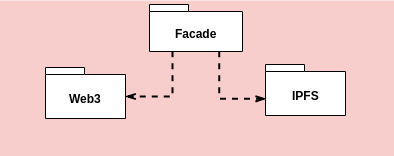
\includegraphics[scale=0.6]{res/images/facade.png}
	\caption{Package diagram with the interaction between facade-web3-IPFS}
\end{figure}

\subsection{Methods}

All the methods described in the picture below consist of two different steps:
\begin{itemize}
	\item \textbf{setter}: first the data is stored to IPFS, then it is stored to Ethereum with the related IPFS CID;
	\item \textbf{getter}: the IPFS CID is retrived from web3. The CID is then used to get the the data from IPFS. 
\end{itemize}


\noindent Since the methods are just a combination of the already described methods of the web3 and IPFS packages, we omit their description.

\subsection{How to extend with new features}
This package should be used to organize information retrieved from different sources before passing them to the front-end. This package hides the interactions between the different technologies, but should not be used to interact directly with the blockchain or IPFS. Two important aspects the developer must keep in consideration are:
\begin{itemize}
	\item if new functionality is added in the Solidity back-end and in the web3 package, the facade package should be updated only if the user could interact directly with this functionality;
	\item even if the purpose of this package is to transform and organize data to make them more readable and usable, it is not responsible for preparing data as they will be shown/used by the front-end, that is containers/actionCreators' responsibility.
\end{itemize}
\begin{figure}[H]
	\centering
	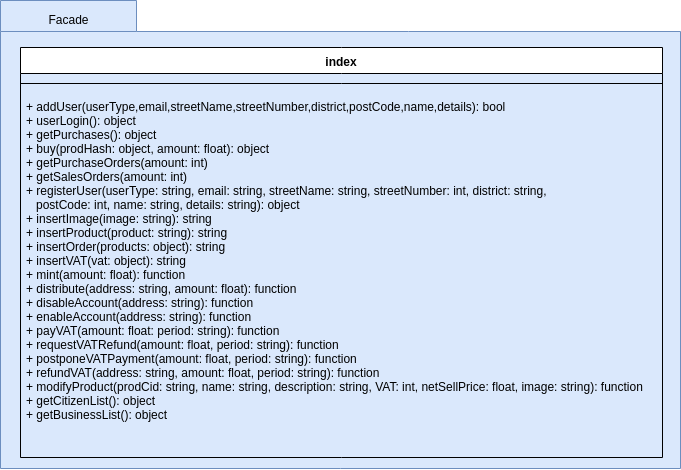
\includegraphics[scale=0.55]{res/images/facade-package.png}
	\caption{Class diagram of the facade package}
\end{figure}

